\chapter{Putting Things Together}
\label{chap:ontology}

This ontology, the Domain Ontology for Instruction, is constituted by the union of the modules described previously, plus % a few global axioms not yet listed with the modules, as well as some
meta-level annotations using the Ontology Design Pattern Representation Language (OPLa) \cite{OPLa,OPLa-tool}.

We consider the controlled vocabularies to be separate from the actual ontology. One advantage of using controlled vocabularies as indicated in this document is, that they provide a seamless capability for expansion of the ontology, by adding further vocabulary items. Sometimes, however, it is the case that there are specific interactions between items in the controlled vocabulary and axioms. % For example, Uagent examples.

Figure \ref{fig:ontology} shows a schema diagram for the combined ontology. % Marked with a red dashed arrow in Figure \ref{fig:ontology} are some suggested \emph{shortcuts} which we discuss further below. An alternative schema diagram for the ontology is given in Figure \ref{fig:ontology-partial}. The main difference to Figure \ref{fig:ontology} is that we removed most of the subclass relationships. 
Please recall that all our schema diagrams are necessarily ambiguous and incomplete -- while they help to understand and use the ontology, it is the set of logical axioms which actually constitutes the ontology.

\begin{figure}[h!]
\begin{center}
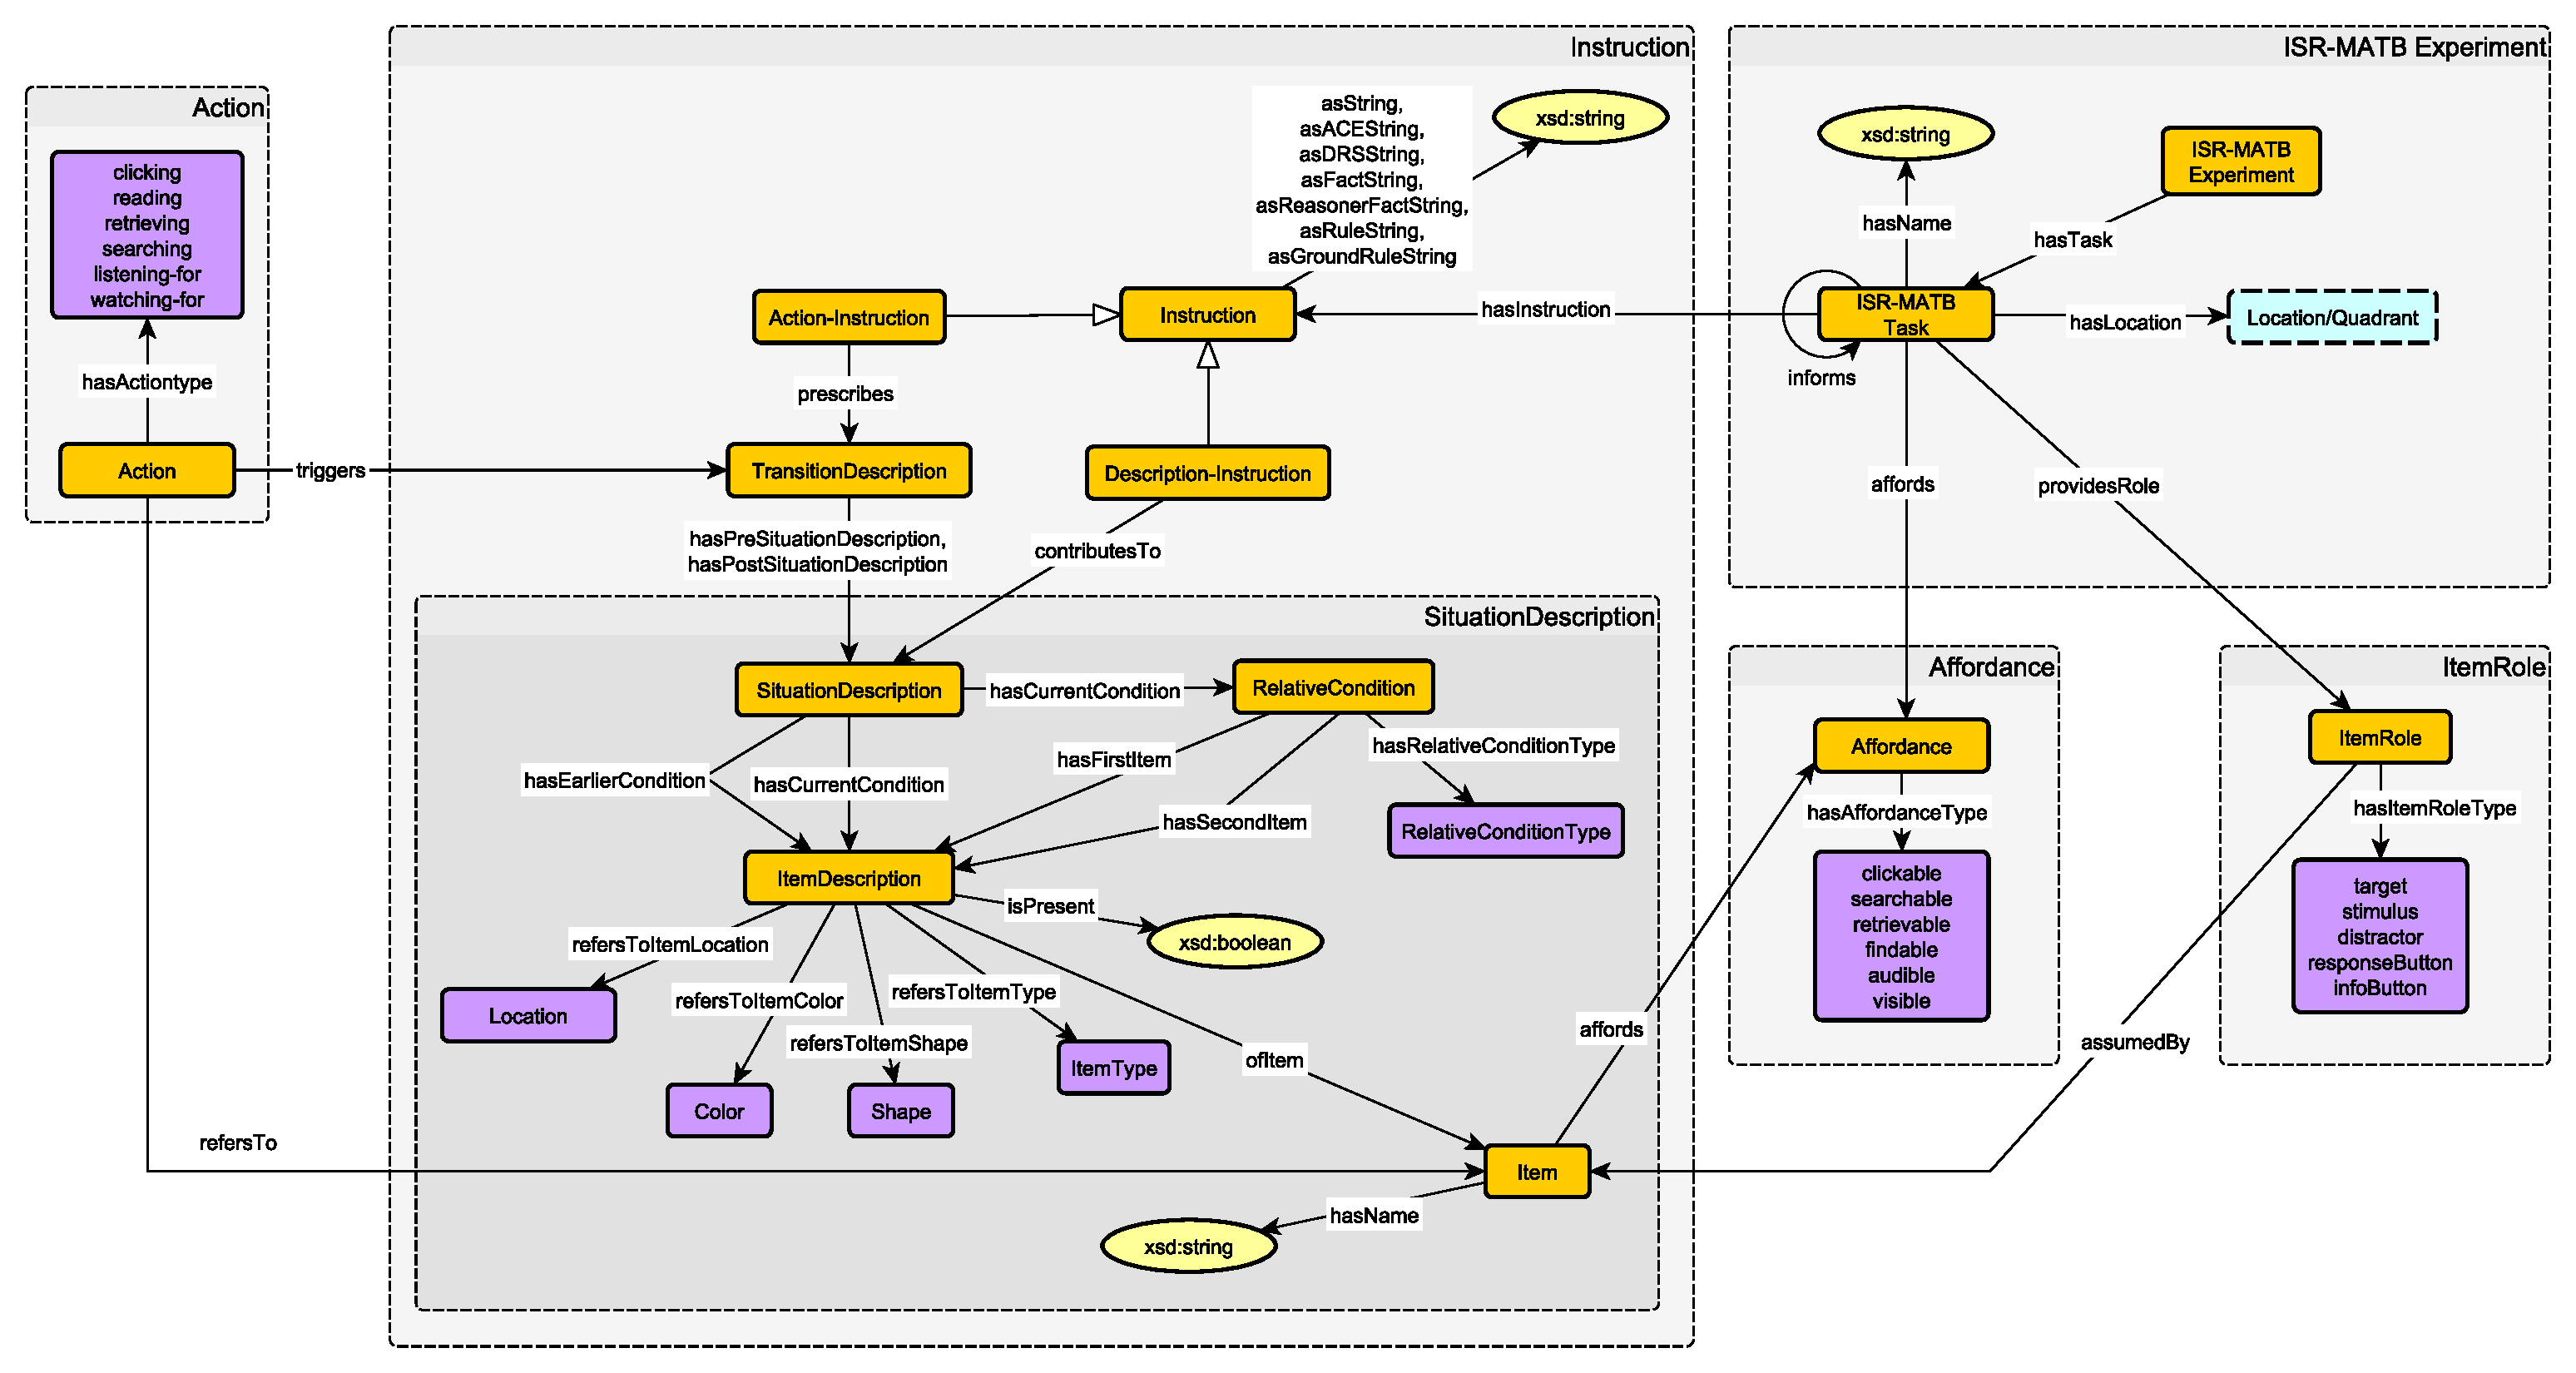
\includegraphics[width=\textwidth]{resources/all-draft-7.pdf}
\end{center}
\caption{Schema Diagram for the combined ontology.}
\label{fig:ontology}
\end{figure}

\section{Axioms}

All axioms belonging to the separate modules are part of the overall ontology. In addition, all pairs of classes which are not declared or inferred to be in a subclass relationship, are declared to be disjoint.

% \section{Shortcuts}

% When working with a complex modular ontology, it is often helpful to provide so-called \emph{shortcuts} \cite{KrisnadhiKHARJ16} which simplify population of the ontology or querying of the underlying knowledge graph in cases where the full complexity of the ontology is not required or needed. 

% Version 1.0 of the Uagent Ontology carries a few such shortcuts which are convenient for population purposes. They are indicated as dashed red arrows in Figure \ref{fig:ontology}. 